\documentclass[english,14pt]{beamer}
\usetheme{EastLansing}
\usecolortheme{spruce}

\usepackage{xcolor}
\usepackage{listings}
\usepackage{courier}
\usepackage{graphicx}
\usepackage{amsmath}
\usepackage{algorithm2e}
\usepackage{multicol}
\usepackage{hyperref}

% http://mirrors.ibiblio.org/CTAN/macros/latex/contrib/datetime2/datetime2.pdf
\usepackage{babel}
\usepackage[useregional]{datetime2}

% https://tex.stackexchange.com/questions/42619/x-mark-to-match-checkmark
\usepackage{pifont}% http://ctan.org/pkg/pifont

%% https://stackoverflow.com/questions/1435837/how-to-remove-footers-of-latex-beamer-templates
%%gets rid of bottom navigation bars
%\setbeamertemplate{footline}[page number]
%
%gets rid of navigation symbols
\setbeamertemplate{navigation symbols}{}


\usefonttheme[onlymath]{serif}

\definecolor{mGreen}{rgb}{0,0.6,0}
\definecolor{mGray}{rgb}{0.5,0.5,0.5}
\definecolor{mPurple}{rgb}{0.8,0,0.82}
\definecolor{backgroundColour}{rgb}{0.95,0.95,0.92}
\definecolor{lightBlue}{rgb}{0.1, 0.1, 0.8}

\newcommand\red[1]{{\color{red} #1}}
\newcommand\green[1]{{\color{green} #1}}
\newcommand\blue[1]{{\color{blue} #1}}

\newcommand{\cmark}{\ding{51}}%
\newcommand{\xmark}{\ding{55}}%

\lstdefinestyle{CStyle}{
    backgroundcolor=\color{backgroundColour},   
    commentstyle=\color{mGreen},
    keywordstyle=\color{magenta},
    numberstyle=\tiny\color{mGray},
    stringstyle=\color{mPurple},
    basicstyle=\footnotesize,
    breakatwhitespace=false,         
    breaklines=true,                 
    captionpos=b,                    
    keepspaces=true,                 
    numbers=left,                    
    numbersep=5pt,                  
    showspaces=false,                
    showstringspaces=false,
    showtabs=false,                  
    tabsize=2,
    language=C
}

\lstdefinestyle{pseudo}{
        basicstyle=\ttfamily\footnotesize,
        keywordstyle=\color{lightBlue},
        morekeywords={BEGIN,END,IF,ELSE,ENDIF,ELSEIF,PRINT,WHILE,RETURN,ENDWHILE,DO,FOR,TO,IN,ENDFOR,BREAK,INPUT},
        morecomment=[l]{//},
        commentstyle=\color{mGreen}
}

\lstset{basicstyle=\footnotesize\ttfamily,breaklines=true}
\lstset{framextopmargin=50pt,tabsize=2}

\title{ENGG1003 - Monday Week 3}
\subtitle{Loops and branching}
\author{Steve Weller}
\institute{University of Newcastle}
%\date{\today}
\date{8 March, 2021}

% following is a bit of a hack, but forces page numbers (technically: frame numbers) to run 1,2,3,... 
% with titlepage counting as frame 1

\addtocounter{framenumber}{1}
\titlepage

\begin{document}

\begin{flushleft}
{\scriptsize Last compiled:~\DTMnow}
\vspace*{-5mm}
\end{flushleft}
\framebreak

%==============================================================

\begin{frame}[fragile]

\frametitle{Lecture overview}
\begin{enumerate}
	\item Iteration using \textbf{\texttt{for}} loop \red{\S3.1}
	\begin{itemize}
		\item fixed number of iterations
	\end{itemize}

	\item[]
	
	\item Iteration using \textbf{\texttt{while}} loop \red{\S3.2}
	\begin{itemize}
		\item keep iterating whenever a condition is satisfied
	\end{itemize}

	\item[]
	
	\item Branching: \textbf{\texttt{if}}, \textbf{\texttt{elif}} and \textbf{\texttt{else}} \red{\S3.3}
	\begin{itemize}
		\item check condition before executing code block
	\end{itemize}
		
\end{enumerate}

\end{frame}

%==============================================================

\begin{frame}[fragile]

\frametitle{$1)$ Iteration using \texttt{for} loop}

\begin{itemize}
	\item many computations for solving engineering problems are intrinsically repetitive
	\item[]
	\item all programming languages have certain \red{\emph{loop}} structures to enable repetitive code execution
	\item[]
	\item Python provides two such structures:
	\begin{itemize}
		\item \texttt{for} loop
		\item \texttt{while} loop
	\end{itemize}
	\item[]
	\vspace*{-3mm}
	\item \textbf{Motivation:} print 5 times table at the console
\end{itemize}

\end{frame}
%==============================================================

\begin{frame}[fragile]

\frametitle{}

\frametitle{Live demo: $5$ times table, brute force}

\begin{figure}[ht]
	\centering
	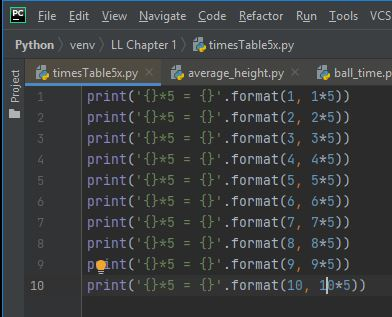
\includegraphics[width=0.5\textwidth]{figures/LLp59aoutput}%
	~~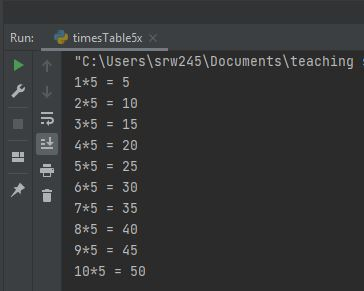
\includegraphics[width=0.5\textwidth]{figures/LLp59boutput}
\end{figure}


\end{frame}

%==============================================================

\begin{frame}[fragile]

\frametitle{Our first loop}

\begin{itemize}
	\item using \texttt{for} loop, can replace $10$ lines of code \\ with just~$2$ lines:
\end{itemize}

\begin{figure}[ht]
	\centering
	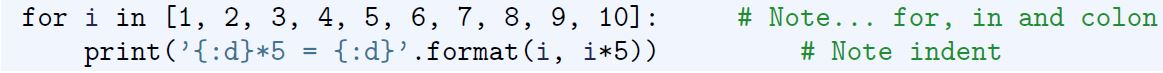
\includegraphics[width=\textwidth]{figures/LLp60b}
\end{figure}

\begin{itemize}
	\item \red{\emph{loop variable}} \texttt{i} takes on each of the values $1$ to $10$
	\item \ldots and for each value the \texttt{print} function is called
\end{itemize}

\end{frame}

%==============================================================

\begin{frame}[fragile]

\frametitle{A typical \texttt{for} loop}

\begin{figure}[ht]
	\centering
	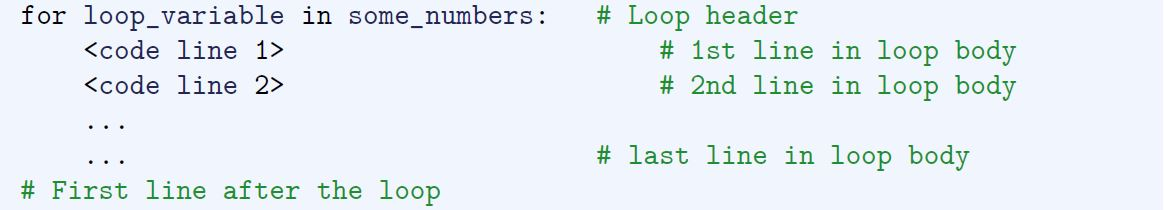
\includegraphics[width=0.9\textwidth]{figures/LLp60c}
\end{figure}
	\vspace*{-3mm}
\begin{itemize}
	\item first line is \red{\emph{for loop header}}
	\begin{itemize}
		\item reserved word \texttt{for}, ends with colon, both necessary
	\end{itemize}
	\item \red{\emph{indented}} lines after header are a \red{\emph{block}} of statements%
	\begin{itemize}
		\item called the \red{\emph{loop body}}
	\end{itemize}
	\item block of code inside a loop \emph{must} be indented 
	\begin{itemize}
		\item indentation is 4 spaces by convention
	\end{itemize}
	\item once indentation is reversed, loop body has ended
\end{itemize}

\end{frame}

%==============================================================

\begin{frame}[fragile]

\frametitle{Nested loops}

\vspace*{-3mm}
\begin{itemize}
	\item for each iteration of a loop\ldots execute \emph{another} loop!
	\item one loop ``inside'' another, hence \red{\emph{nested}}
	\item \emph{two} levels of indentation are needed
\end{itemize}
	
\begin{figure}[ht]
	\centering
	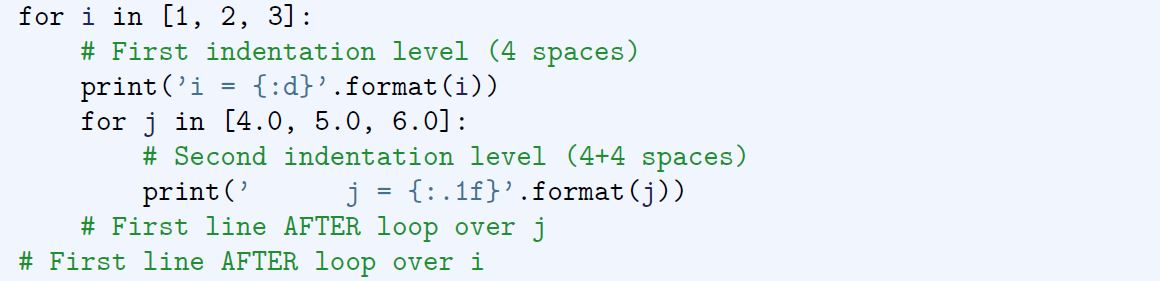
\includegraphics[width=0.75\textwidth]{figures/LLp61a}
\end{figure}
\vspace*{-3mm}
\begin{figure}[ht]
	\centering
	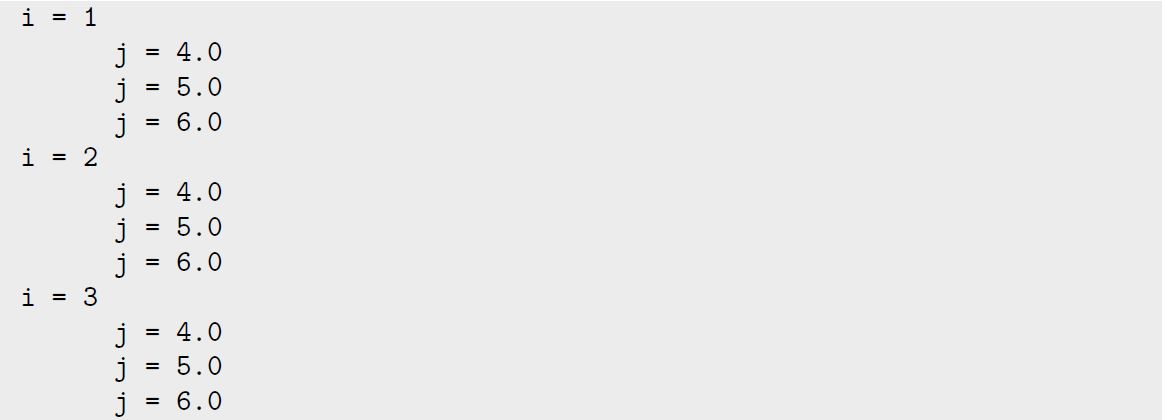
\includegraphics[width=0.75\textwidth]{figures/LLp61b}
\end{figure}

\end{frame}

%==============================================================

\begin{frame}[fragile]

\frametitle{Combining \texttt{for} loop and \texttt{array}}

\begin{itemize}
	\item elements of each \texttt{array} are identified by an index
	\item \texttt{for} loop can use array index as a loop variable
\end{itemize}
\vspace*{2mm}
\textbf{Example:}~compute average of five numbers
\[
\frac{h[\red{0}] + h[\red{1}] + h[\red{2}] + h[\red{3}] + h[\red{4}]}{5}
\]
\vspace*{-6mm}
\begin{figure}[ht]
	\centering
	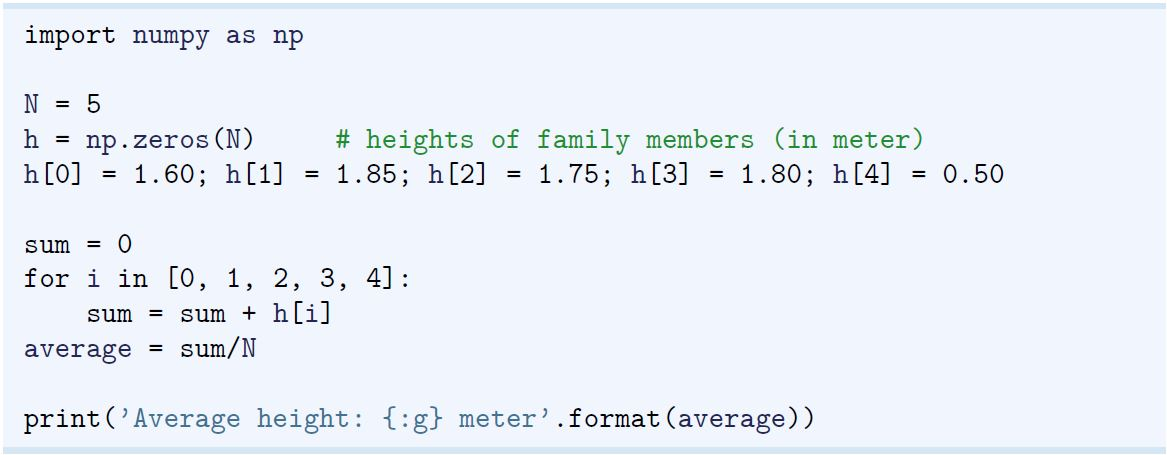
\includegraphics[width=0.75\textwidth]{figures/LLp62a}
\end{figure}

\end{frame}

%==============================================================

\begin{frame}[fragile]

\frametitle{Live demo: \texttt{for} loop}

\begin{itemize}
	\item Python code:~\href{https://github.com/slgit/prog4comp_2/blob/master/py36-src/average_height.py}{\texttt{average\_height.py}}
\end{itemize}

\end{frame}

%==============================================================

\begin{frame}[fragile]

\frametitle{Using the \texttt{range} function}

\begin{itemize}
	\item what about \texttt{for} loop with \emph{really large} number of iterations?
	\begin{itemize}
		\item[\red{\xmark}] \texttt{for i in [0,1,2,3,4, \ldots, 9999]:}
	\end{itemize}
	
	\item built-in function \texttt{range} solves this problem
	
	\item instead of \verb+for i in [0, 1, 2, 3, 4]:+

	\item[] \ldots use this~ \verb+for i in range(0, 5, 1):+
	
	\item general form of call to \texttt{range} as follows
	\begin{figure}[ht]
		\centering
		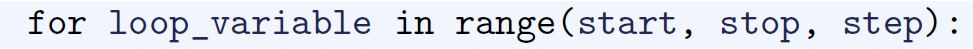
\includegraphics[width=0.75\textwidth]{figures/LLp64c}
	\end{figure}
	\item[]%
	\begin{itemize}
		\item start at integer \texttt{start}
		\item[] \qquad\ldots increment by integer \texttt{step}
		\item[] \qquad\qquad\ldots stop before integer \texttt{stop}
	\end{itemize}

\end{itemize}

\end{frame}

%==============================================================

\begin{frame}[fragile]

\frametitle{$2)$ Iteration using \texttt{while} loop}

\begin{itemize}
	\item \texttt{for} loop runs for a specified number of iterations

	\item[]
	
	\item second basic loop construction in Python is the \texttt{while} loop
	\begin{itemize}
		\item runs as long as a \red{\emph{condition}} is~\texttt{True}
	\end{itemize}
	
	\item[]
	
	\item how do we write ``conditions'' in Python?
	\item how do we decide a condition is \texttt{True} or \texttt{False}?
\end{itemize}

\end{frame}

%==============================================================

\begin{frame}[fragile]

\frametitle{Boolean expressions}
	
\begin{itemize}
	\item in programming, often need to check whether something is true or not true
	\begin{itemize}
		\item \ldots and take action accordingly
		\item[] eg: mass loading on bridge $< 30,000$~kg?
		\item[] eg: pH in a tank above $10$?
	\end{itemize}
	
	\item handled using \red{\emph{logical}} or \red{\emph{Boolean expressions}}

	\item these evaluate to \red{\emph{Boolean values}} \texttt{True} and \texttt{False}
	\begin{itemize}
		\item note capital letters T and F
	\end{itemize}
	\item  six \red{\emph{relational operators}} to compare values in Python
	
	\item[]	\begin{itemize}[]
		\begin{tabular}{llll}
		\textbf{\texttt{>}} 	&  greater than\qquad\qquad 	& \textbf{\texttt{>=}} 	& greater than or equal to \\
		\textbf{\texttt{<}} 	&  less than\qquad\qquad 		& \textbf{\texttt{<=}} 	& less than or equal to \\						\textbf{\texttt{==}} 	&  equal to\qquad\qquad 		& \textbf{\texttt{!=}} 		& not equal to
		\end{tabular}
	\end{itemize}
	 
\end{itemize}

\end{frame}

%==============================================================

\begin{frame}[fragile]

\frametitle{Comparing values}

Live demo

\begin{figure}[ht]
	\centering
	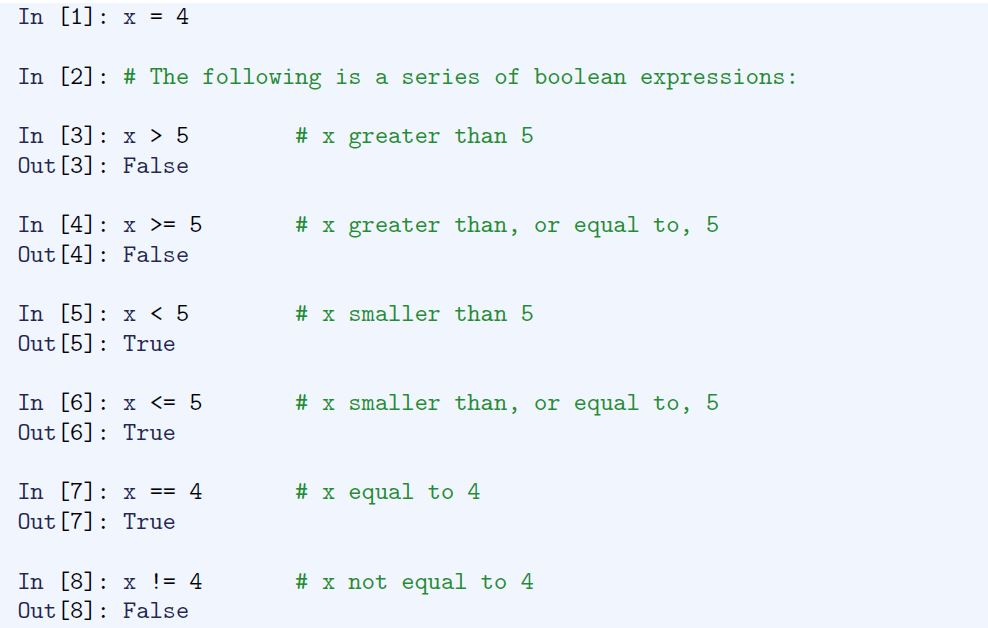
\includegraphics[width=0.8\textwidth]{figures/LLp46}
\end{figure}
	
\end{frame}

%==============================================================

\begin{frame}[fragile]

\frametitle{Boolean operators: \texttt{and}, \texttt{or}, \texttt{not}}

Live demo 

\begin{figure}[ht]
	\centering
	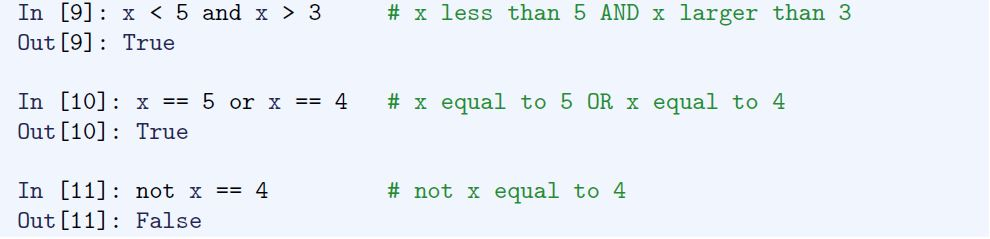
\includegraphics[width=0.9\textwidth]{figures/LLp47a}
\end{figure}

\begin{itemize}
	\item Boolean variable type
	\begin{itemize}
		\item int, float, str, \textbf{\red{bool}}
	\end{itemize}

	\item Boolean values may be combined into longer expressions using \texttt{and}, \texttt{or} and \texttt{not}

	\item basics of Boolean operators:~week 1 Thurs lecture
	\begin{itemize}
		\item covered in \emph{much} more depth in ELEC1710
	\end{itemize}
\end{itemize}

\end{frame}

%==============================================================

\begin{frame}[fragile]

\frametitle{Example: Finding the time of flight}

\begin{itemize}
	\item illustrate \texttt{while} loop by modifying earlier ``soccer ball'' example
	\item[]
	\item initial velocity of ball is slightly lower, only $4.5$~m/s
	\begin{itemize}
		\item was $5$~m/s in last weeks lecture
	\end{itemize}
	\item[]
	\item[]\textbf{Goal:} compute how long ball is in the air
\end{itemize}

\end{frame}

%==============================================================

\begin{frame}[fragile]

\frametitle{Ball height vs.\ time}

\begin{figure}[ht]
	\centering
	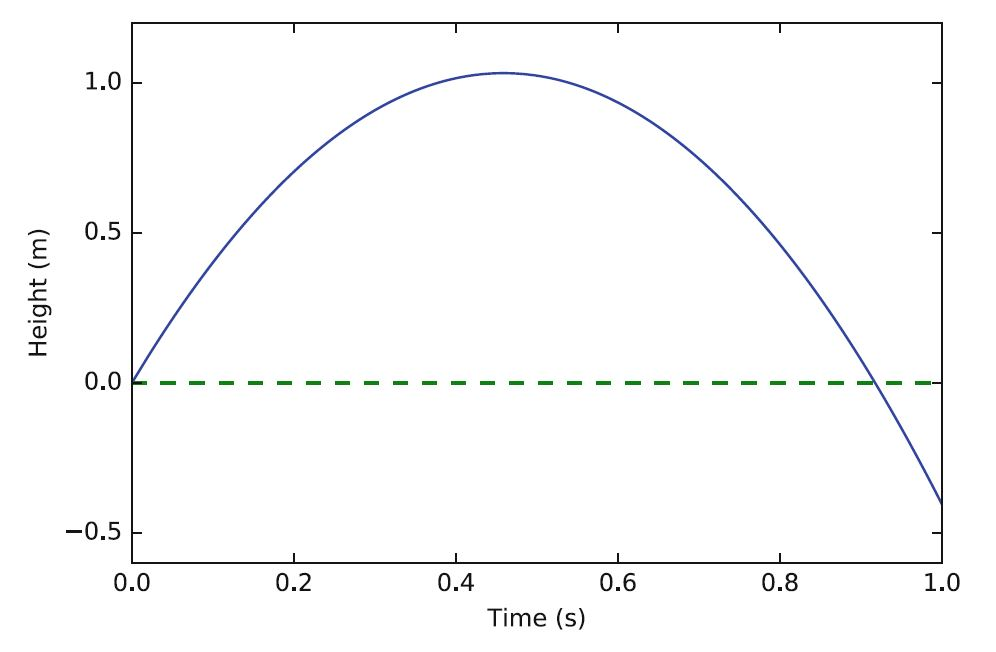
\includegraphics[width=0.7\textwidth]{figures/LLp66output}
\end{figure}

\vspace*{-5mm}
\begin{itemize}
	\item height is eventually \emph{negative}, ie: for large enough~$t$
	\item \textbf{Idea:} find smallest $t$ where height $y(t) < 0$
\end{itemize}
	
\end{frame}

%==============================================================

\begin{frame}[fragile]

\frametitle{}

\begin{figure}[ht]
	\centering
	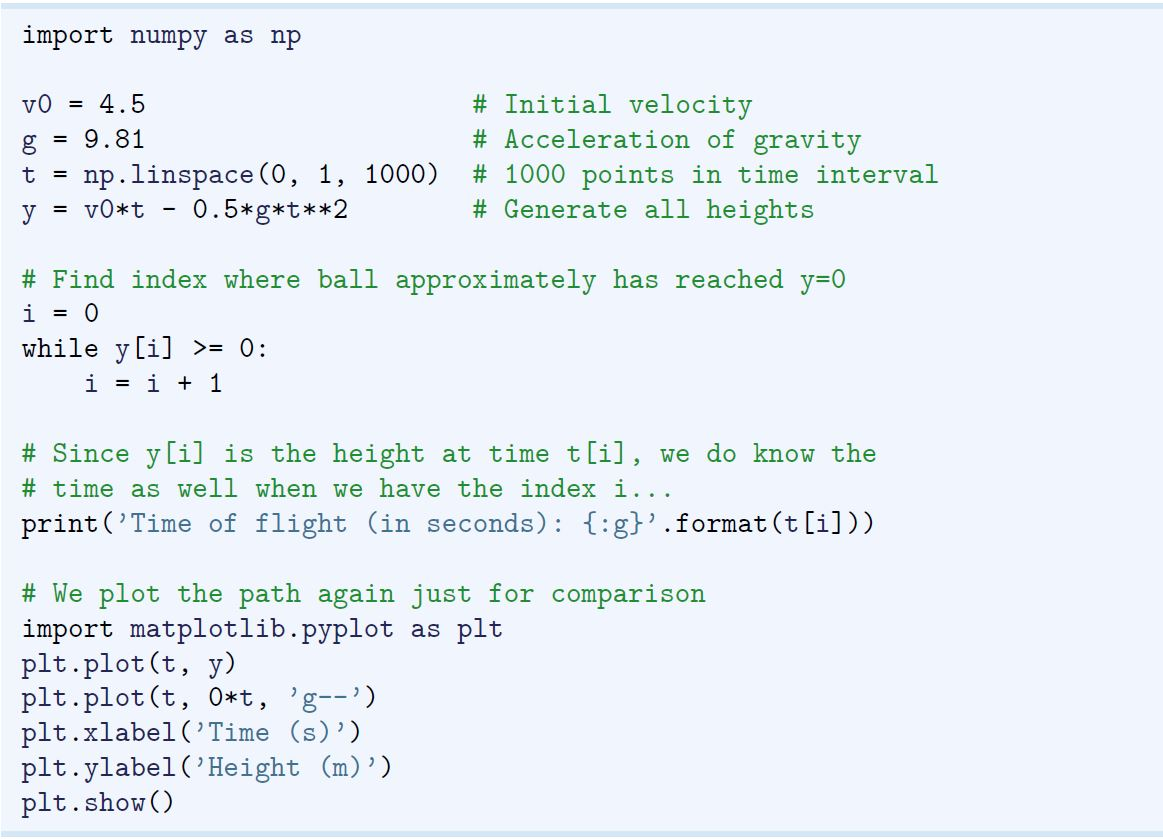
\includegraphics[width=0.9\textwidth]{figures/LLp65a}
\end{figure}
\vspace*{-3mm}
Python code:~\href{https://github.com/slgit/prog4comp_2/blob/master/py36-src/ball_time.py}{\texttt{ball\_time.py}}

\end{frame}

%==============================================================

\begin{frame}[fragile]

\frametitle{}

\begin{figure}[ht]
	\centering
	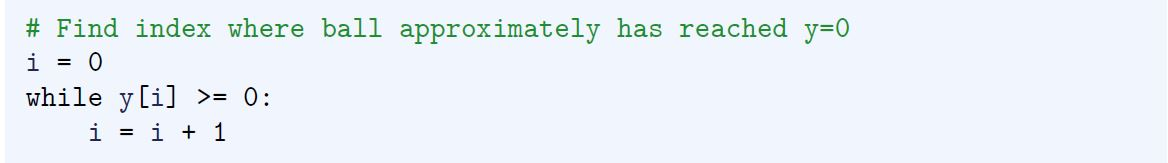
\includegraphics[width=0.9\textwidth]{figures/LLp65b}
\end{figure}

\vspace*{-5mm}
\begin{itemize}
	\item loop index \texttt{i} inialised at \texttt{0}
	\begin{itemize}
		\item interested in heights \texttt{y[0], y[1], y[2], \ldots} \\ at times \texttt{t[0], t[1], t[2], \ldots}
	\end{itemize}
	\item loop runs as long as condition \texttt{y[i] >= 0} evaluates to \texttt{True}
	\begin{itemize}
		\item \ldots and index \texttt{i} is incremented by $1$
		\item checks successive elements in array \texttt{y}
	\end{itemize}
	\item when \texttt{y[i] >= 0} evaluates to \texttt{False}
	\item[] \ldots we've found the first height that is negative!
	\item loop terminates and code \emph{after} loop is executed
	\item \texttt{i} is smallest index for which height \texttt{y[i] < 0}

\end{itemize}

\end{frame}

%==============================================================

\begin{frame}[fragile]

\frametitle{}

\begin{figure}[ht]
	\centering
	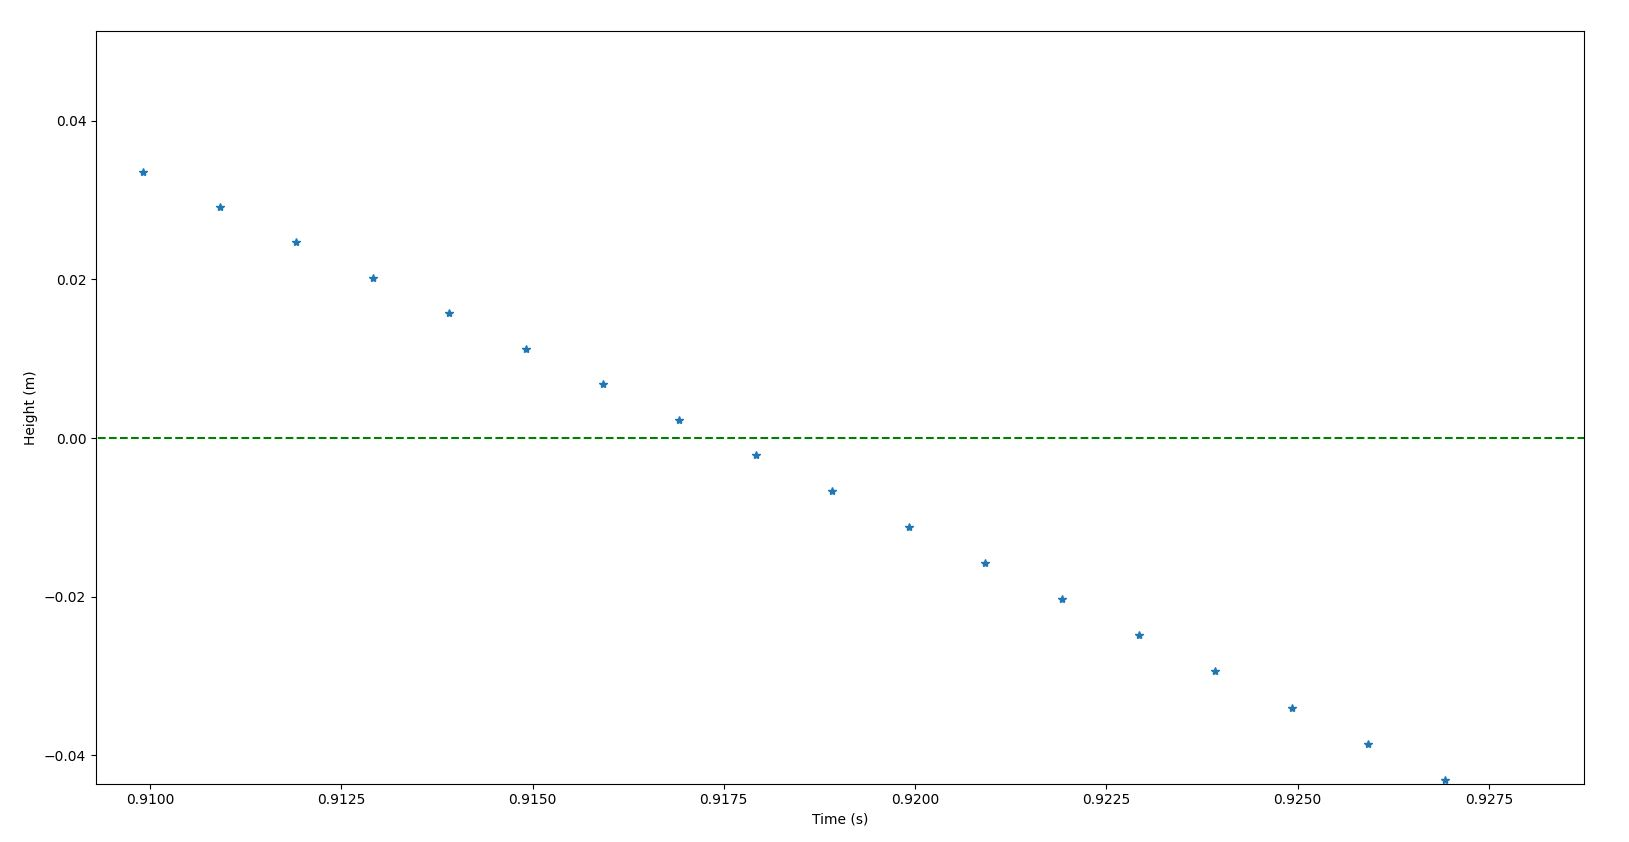
\includegraphics[width=0.9\textwidth]{figures/LLp66ZoomOutput}
\end{figure}
\vspace*{-5mm}
\begin{itemize}
	\item \texttt{i} $= 917$
	\item \texttt{y[916]} $= 0.002312$
	\item \texttt{y[917]} $= -0.002190$
\end{itemize}

\end{frame}

%==============================================================

\begin{frame}[fragile]

\frametitle{Structure of a typical \texttt{while} loop}

\begin{figure}[ht]
	\centering
	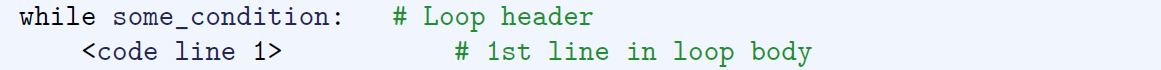
\includegraphics[width=\textwidth]{figures/LLp66a}
	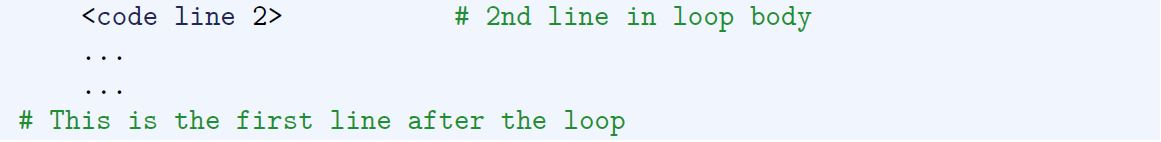
\includegraphics[width=\textwidth]{figures/LLp67a}
\end{figure}
\vspace*{-3mm}
\begin{itemize}
	\item first line is \red{\emph{while loop header}}
	\begin{itemize}
		\item reserved word \texttt{while}, ends with colon, both necessary
	\end{itemize}
	\item indented lines after header are a \red{\emph{block}} of statements%
	\begin{itemize}
		\item called the \red{\emph{loop body}}
	\end{itemize}
	\item indentation is 4 spaces by convention
	\item once indentation is reversed, loop body has ended
\end{itemize}

\end{frame}

%==============================================================

\begin{frame}[fragile]

\frametitle{}

\begin{itemize}
	\item \texttt{some\_condition} is a Boolean expression
	\begin{itemize}
		\item must evaluate to \texttt{True} or \texttt{False}
	\end{itemize}
	
	\item[]
	
	\item if \texttt{some\_condition} is initially \texttt{False}:
	\begin{itemize}
		\item loop body statements are \emph{never} executed
	\end{itemize}

	\item[]
	
	\item if \texttt{some\_condition} is initially \texttt{True}:
	\begin{itemize}
		\item statements in loop body are evaluated once
		\item[] \qquad\texttt{some\_condition} evaluated again
		\item[] \qquad\qquad \ldots and the process continues
	\end{itemize}
	
	\item[]
	
	\item[] \textbf{Summary:}~\texttt{while} loop runs until the Boolean expression \texttt{some\_condition} becomes \texttt{False}
\end{itemize}

\end{frame}

%==============================================================

\begin{frame}[fragile]

\frametitle{Infinite loops}

\begin{itemize}
	\item Possible to have a \texttt{while} loop in which the condition \emph{never} evaluates to \texttt{False}
	\begin{itemize}
		\item program execution cannot escape the loop!
	\end{itemize}
	
	\item[]
	
	\item Referred to as an \red{\emph{infinite loop}}
	
	\item[]
	
	\item Might be deliberate \ldots
	\begin{itemize}
		\item program runs ``forever'', eg: surveillance camera system
	\end{itemize}
	
	\item[]
	\item \ldots but infinite loops are usually unintentional
	\begin{itemize}
		\item result of a program \red{\emph{bug}}
		\item \texttt{Ctrl+c} to stop program
	\end{itemize}
	
\end{itemize}

\end{frame}

%==============================================================

\begin{frame}[fragile]

\frametitle{$3)$ Branching:~\texttt{if}, \texttt{elif} and \texttt{else}}

\begin{itemize}
	\item[] \textbf{Aim:} write a program that helps us decide whether we should go swimming or not
	\begin{itemize}
		\item based on water temperature in degrees Celcius ($^\circ$C)
	\end{itemize}
	\item[]
	\item will build up a program in stages
	\begin{itemize}
		\item programming as a step-wise process
	\end{itemize}
\end{itemize}

\end{frame}

%==============================================================

\begin{frame}[fragile]

\frametitle{One \texttt{if}-test}

\begin{figure}[ht]
	\centering
	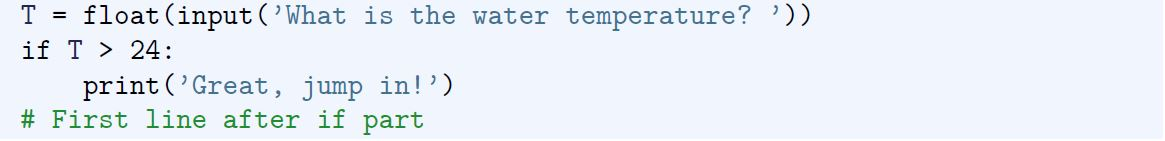
\includegraphics[width=\textwidth]{figures/LLp68a}
\end{figure}
\vspace*{-3mm}
\begin{itemize}
	\item \texttt{T = float(input(\ldots}
	\begin{itemize}
		\item reads string from console, and converts to float \texttt{T}
	\end{itemize}
	\item[]
	\item if $T > 24$, then string is printed
	\item[]
	\item \ldots and if $T \leq  24$ then
	\begin{itemize}
		\item print command is \emph{not} executed
		\item program continues to \texttt{\# First line after if part}
	\end{itemize}
\end{itemize}

\end{frame}

%==============================================================

\begin{frame}[fragile]

\frametitle{Two \texttt{if}-tests}

\begin{figure}[ht]
	\centering
	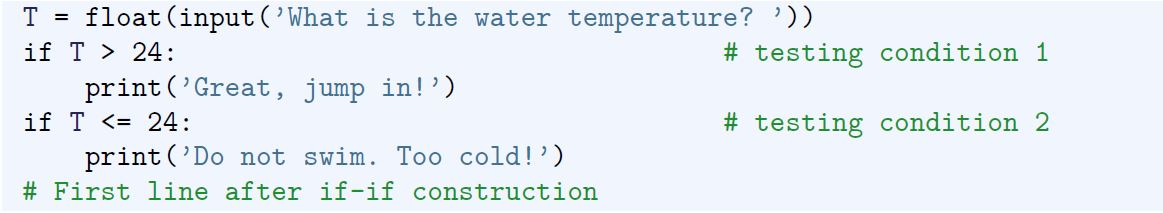
\includegraphics[width=\textwidth]{figures/LLp68b}
\end{figure}
\vspace*{-3mm}
\begin{itemize}
	\item precisely one of the following two strings is displayed:
	\begin{itemize}
		\item ``Great, jump in!''
		\item ``Do not swim. Too cold!''
	\end{itemize}
	
\end{itemize}

\end{frame}

%==============================================================

\begin{frame}[fragile]

\frametitle{An \texttt{if}-\texttt{else} construction}

\begin{itemize}
	\item since the conditions are \red{\emph{mutually exclusive}}
	\begin{itemize}
		\item $T > 24$
		\item $T \leq 24$
	\end{itemize}
	\item we can simplify code with \texttt{if}-\texttt{else}
\end{itemize}
	
\begin{figure}[ht]
	\centering
	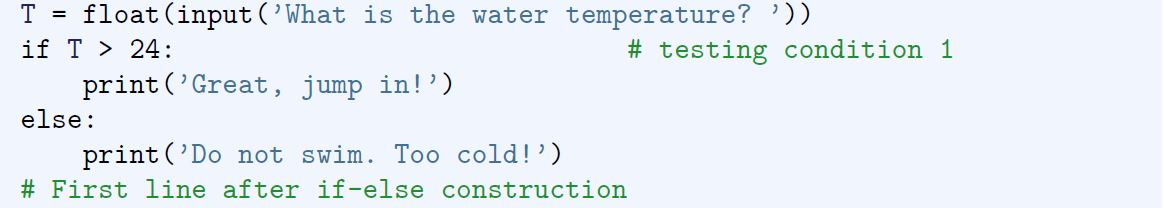
\includegraphics[width=\textwidth]{figures/LLp69a}
\end{figure}

\end{frame}

%==============================================================

\begin{frame}[fragile]

\frametitle{An \texttt{if}-\texttt{elif}-\texttt{else} construction}

\begin{figure}[ht]
	\centering
	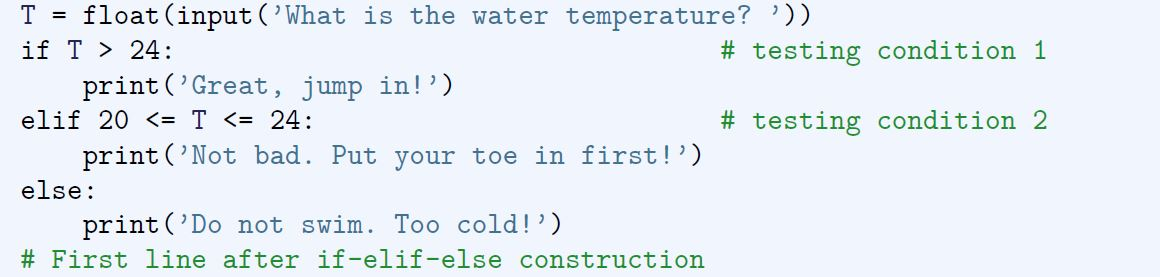
\includegraphics[width=\textwidth]{figures/LLp69b}
\end{figure}

\begin{itemize}
\item final enhancement of program has advice for \emph{three} temperature categories:
	\begin{itemize}
		\item $T > 24$
		\item $20 \leq T \leq 24$
		\item $T < 20$
	\end{itemize}
	\item $T < 20$ condition is captured by \texttt{else}
\end{itemize}

\end{frame}

%==============================================================

\begin{frame}[fragile]

\frametitle{General form of an \texttt{if}-\texttt{elif}-\texttt{else}}

\begin{figure}[ht]
	\centering
	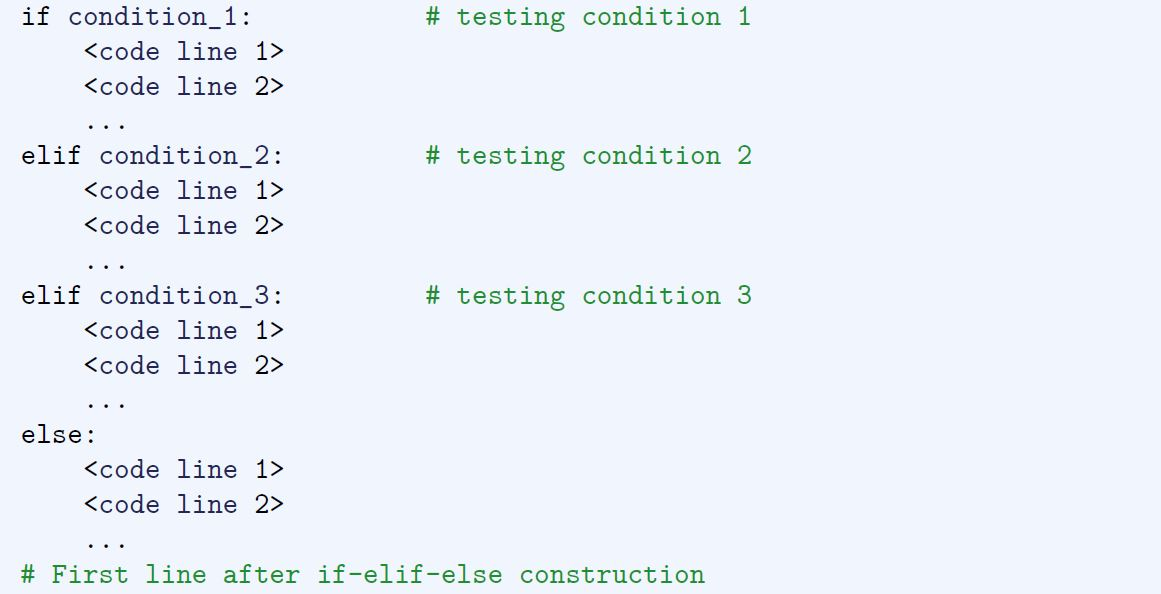
\includegraphics[width=\textwidth]{figures/LLp70a}
\end{figure}

\end{frame}

%%==============================================================
%
%\begin{frame}[fragile]
%
%\frametitle{Example: Finding the Maximum Height}
%
%\begin{itemize}
%	\item excellent illustration of further mod to ball plot
%	\item \textbf{but save this for Thursday lecture}
%	\item can solve in two ways: both shown on p71
%\end{itemize}
%
%\end{frame}

%==============================================================

\begin{frame}[fragile]

\frametitle{Lecture summary}
\begin{itemize}
	\item Iteration using \textbf{\texttt{for}} loop
	\begin{itemize}
		\item fixed number of iterations
	\end{itemize}

	\item[]
	
	\item Iteration using \textbf{\texttt{while}}
		\begin{itemize}
			\item keep iterating whenever a Boolean condition is satisfied
		\end{itemize}

	\item[]
	
	\item Branching: \textbf{\texttt{if}}, \textbf{\texttt{elif}} and \textbf{\texttt{else}}
		\begin{itemize}
			\item conditional execution of code blocks
			\begin{itemize}
				\item \texttt{if}
				\item \texttt{if}-\texttt{else}
				\item \texttt{if}-\texttt{elif}-\texttt{else}
			\end{itemize}
		\end{itemize}
		
\end{itemize}

\end{frame}

\end{document}